\documentclass{beamer}
\usepackage{graphicx}
\usepackage{setspace}
\usepackage{dirtytalk}

\usetheme{Singapore}

\setbeamertemplate{frametitle}[default][center]
\setbeamercolor{frametitle}{fg=black}
\setbeamertemplate{navigation symbols}{}
\setbeamertemplate{footline}[frame number]

\renewcommand*{\thefootnote}{\fnsymbol{footnote}}

\setstretch{1.3}

\begin{document}

\begin{frame}{Inteligenţa artificială şi învăţarea automată}
\begin{center}
	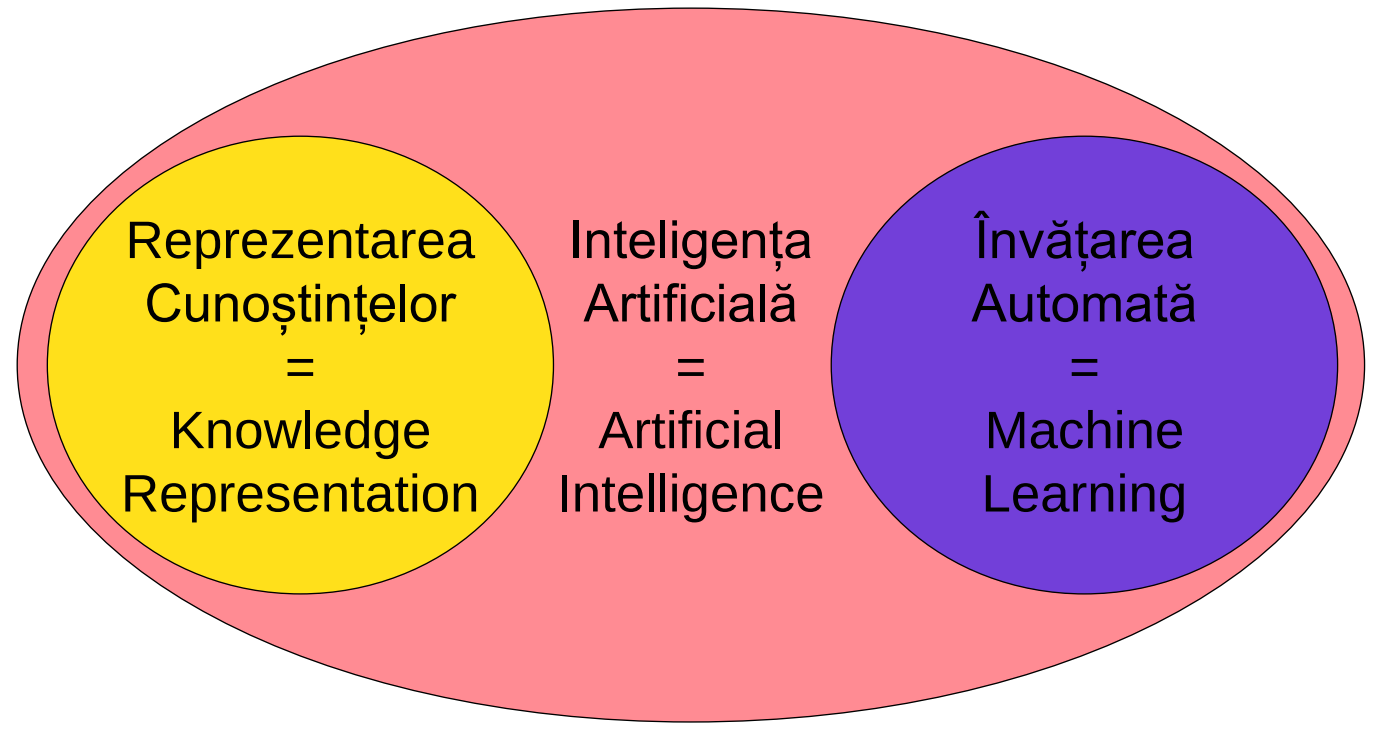
\includegraphics[scale=.21]{pic1.png}
\end{center}
\end{frame}

\begin{frame}{La ce se referă inteligența artificială?}
\begin{itemize}
	\item[$\bullet$] Scopul suprem al inteligenței artificiale este de a construi sisteme care să atingă nivelul de inteligență al omului
	\item[$\bullet$] Testul Turing: un computer prezintă un nivel de inteligență uman dacă un interlocutor uman nu reușește să distingă, în urma unei
conversații în limbaj natural, că vorbește cu un om sau cu un
calculator
\end{itemize}

\begin{center}
	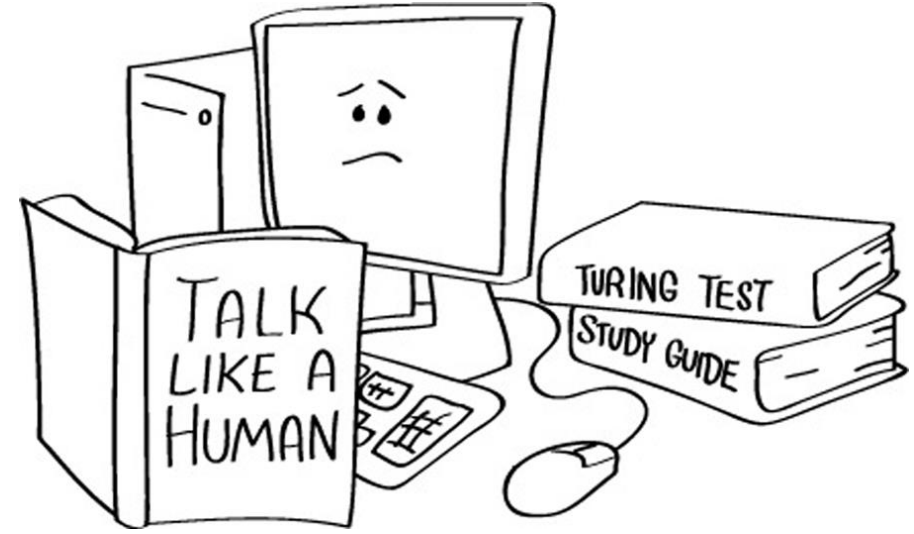
\includegraphics[scale=.19]{pic2.png}
\end{center}
\end{frame}

\begin{frame}{La ce se referă învățarea automată?}
\begin{itemize}
	\item[$\bullet$] O mare parte din cercetători consideră că acest scop poate fi atins prin imitarea modului în care o oamenii învață
	\item[$\bullet$] \textbf{Învățarea automată} – domeniu care studiază modul în care calculatoarele pot fi înzestrate cu abilitatea de a învăța, fără ca aceasta să fie programată în mod explicit
	\item[$\bullet$] În acest context, \textbf{învățarea} se referă la recunoașterea unor tipare / structuri (patterns) complexe și la luarea deciziilor inteligente bazate pe observațiile din \textbf{date}
\end{itemize}
\end{frame}

\begin{frame}{Problemă \say{bine pusă} de învăţare automată}
\begin{itemize}
	\item[$\bullet$] Ce probleme pot fi rezolvate\footnote{rezolvate cu un anumit grad de acuratețe} folosind învățarea automată?
	\item[$\bullet$] \textbf{Problemă \say{bine pusă} de învățare automată:}
	\item[$\bullet$] Spunem despre un program pe calculator că învață dintr-o experiență E în raport cu o clasă de task-uri T și o măsură de performanță P, dacă performanța sa în rezolvarea taskurilor T, măsurată prin P, se îmbunătățește odată cu experiența E
\end{itemize}
\end{frame}

\begin{frame}{Problemă \say{bine pusă} de învăţare automată}
\begin{itemize}
	\item[$\bullet$] Arthur Samuel (1959) a scris un program pentru a juca dame (probabil primul program bazat pe conceptul de învățare)
	\item[$\bullet$] Programul a jucat împotriva lui însuși 10 mii de jocuri
	\item[$\bullet$] Programul a fost conceput să găsească ce poziții ale tablei de joc erau bune sau rele în funcție de probabilitatea de a câștiga sau pierde
\end{itemize}

\begin{columns}
\begin{column}{0.5\textwidth}
	\begin{itemize}
		\item[$\bullet$] În acest caz:
		\item[$\bullet$] E = 10000 de jocuri
		\item[$\bullet$] T = joacă dame
		\item[$\bullet$] P = dacă câștigă sau nu
	\end{itemize}
\end{column}
\begin{column}{0.4\textwidth}
    \begin{center}
	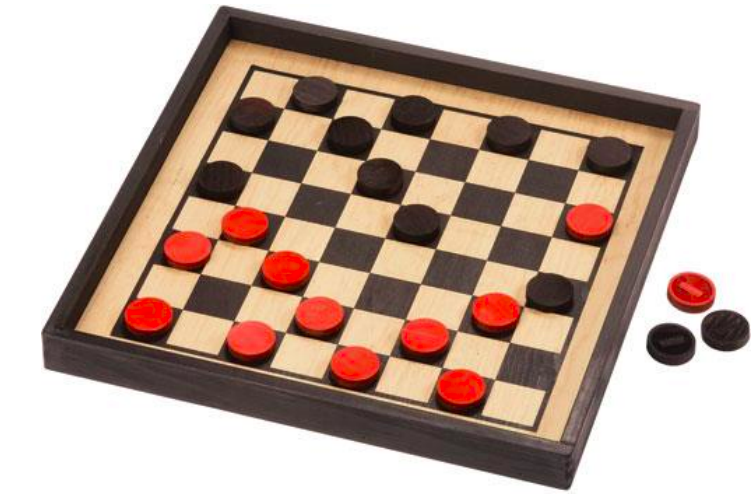
\includegraphics[scale=.15]{pic3.png}
     \end{center}
\end{column}
\end{columns}
\end{frame}

\begin{frame}{Când se aplică învățarea automată?}
\begin{itemize}
	\item[$\bullet$] Se aplică în situații în care este foarte greu (imposibil) să definim un set de reguli de mână / să scriem un program
	\item[$\bullet$] Exemple de probleme unde putem aplica învățarea automată:
	\item[$\bullet$] Detectarea facială
	\item[$\bullet$] Înțelegerea vorbirii
	\item[$\bullet$] Prezicerea prețului acțiunilor
	\item[$\bullet$] Recunoașterea obiectelor
\end{itemize}
\end{frame}

\begin{frame}{Esența învățării automate}
\begin{itemize}
	\item[$\bullet$] Există un tipar
	\item[$\bullet$] Dar nu îl putem exprima programatic / matematic
	\item[$\bullet$] Avem date / exemple în care regăsim acest tipar
\end{itemize}
    \begin{center}
	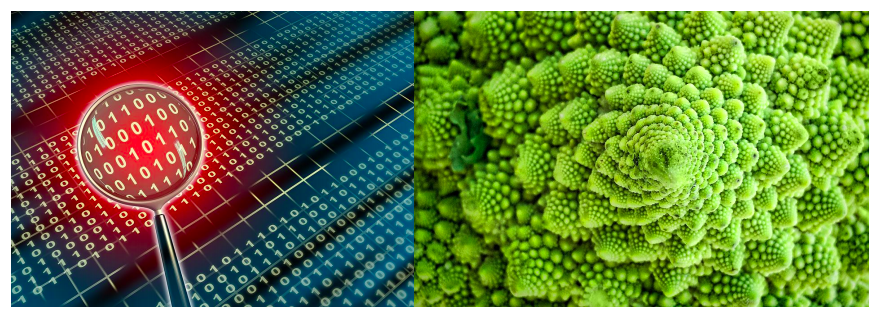
\includegraphics[scale=.35]{pic4.png}
     \end{center}
\end{frame}

\begin{frame}{}
\begin{center}
	{\huge Programare tradițională}
	\\[.5cm]
	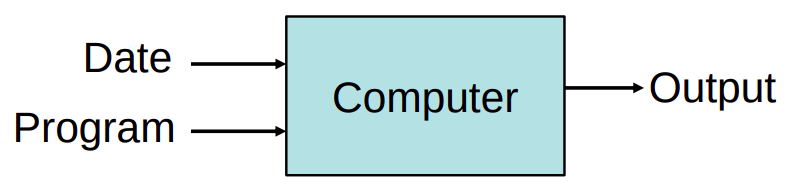
\includegraphics[scale=.35]{pic5.png}
	\\[.5cm]
	{\huge Învăţare automată}
	\\[.5cm]
	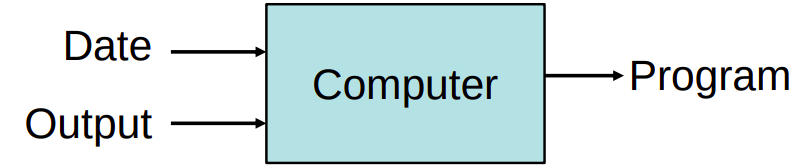
\includegraphics[scale=.35]{pic6.png}
\end{center}
\end{frame}

\begin{frame}{Scurt istoric al inteligenței artificiale}
\begin{itemize}
	\item[$\bullet$] Anii 1960-1980: \say{AI Winter}
	\item[$\bullet$] Anii 1990: Rețelele neuronale domină, în principal datorită descoperirii algoritmului de propagare a erorii înapoi pentru rețele cu mai multe straturi
	\item[$\bullet$] Anii 2000: Metodele kernel domină, în principal din cauza instabilității rețelelor neuronale
	\item[$\bullet$] Anii 2010: Revenirea la rețele neuronale, în principal datorită conceptului de învățare profundă (deep learning)
\end{itemize}
\end{frame}

\begin{frame}{De ce funcționează în prezent?}
\begin{columns}
\begin{column}{0.4\textwidth}
	\begin{itemize}
		\item[$\bullet$] Mai multă putere de calcul
		\item[$\bullet$] Mai multe date
		\item[$\bullet$] Modele mai bune
	\end{itemize}
\end{column}
\begin{column}{0.5\textwidth}
    \begin{center}
	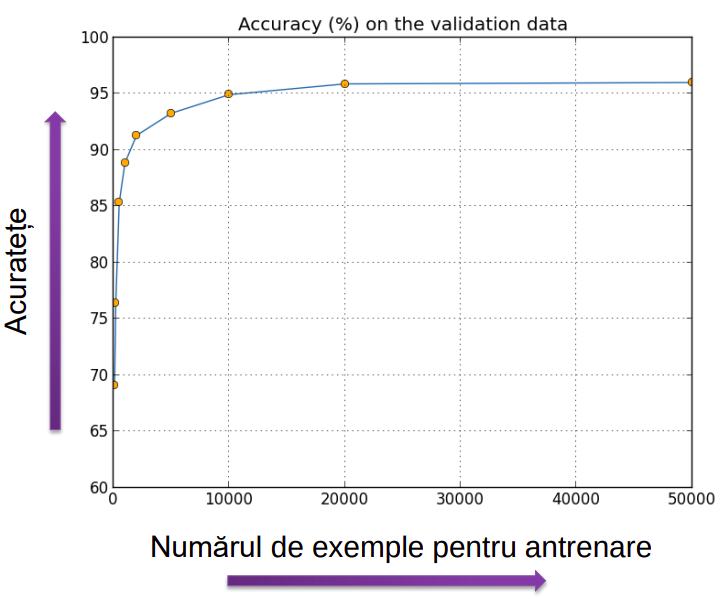
\includegraphics[scale=.24]{pic7.png}
     \end{center}
\end{column}
\end{columns}
\end{frame}

\begin{frame}{Esența învățării automate}
\begin{itemize}
	\item[$\bullet$] Mii de algoritmi de învățare automata existenți
	\item Cercetătorii publică sute de noi algoritmi în fiecare an
	\item[$\bullet$] Simplificând decenii de cercetare în domeniu, putem reduce învățarea automată la:
	\item Învățarea unei funcții $f$ care să mapeze un input $X$ către un output $Y$, anume $f:X \to Y$
	\item Exemplu: $X$: email-uri, $Y$: \{spam, non-spam\}
\end{itemize}
\end{frame}

\begin{frame}{Esența învățării automate}
\begin{itemize}
	\item[$\bullet$] Input: $X$ \hfill (imagini, texte, email-uri...)
	\item[$\bullet$] Output: $Y$ \hfill (spam sau non-spam...)
	\item[$\bullet$] Funcţia Target (necunoscută)\\
	$f:X\to Y$ \hfill (realitatea / \say{adevărata} mapare)
	\item[$\bullet$] Date\\
	$(x_1, y_1), (x_2, y_2), \ldots (x_N, y_N)$
	\item[$\bullet$] Model\\
	$g : X \to Y$\\
	$y = g(x) = sign(w^Tx)$
\end{itemize}
\end{frame}

\begin{frame}{Esența învățării automate}
\begin{itemize}
	\item[$\bullet$] Orice algoritm de învăţare automată are 3 componente:
	\item Reprezentare / Modelare
	\item Evaluare / Funcţie obiectiv
	\item Optimizare
\end{itemize}
\end{frame}

\begin{frame}{Ce cunoştinţe sunt necesare?}
\begin{center}
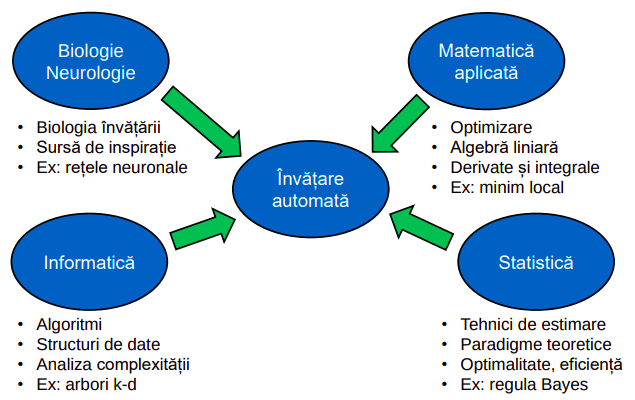
\includegraphics[scale=.45]{pic8.png}
\end{center}
\end{frame}

\end{document}
